\documentclass[runningheads]{llncs}
%
\usepackage{graphicx}
\usepackage{amssymb}
\usepackage{amsmath}
\usepackage{hyperref}
\usepackage{float}
\usepackage{xcolor}
\usepackage{svg}
\usepackage[parfill]{parskip}


\begin{document}
%
\title{Learning Causal Knowledge Graphs from Text Log Data}
%
\author{Aleksandr Eismont}
\institute{Karlsruhe Institute of Technology, Kaiserstr. 12, 76131 Karlsruhe, Germany
\email{ukqln@student.kit.edu}}
%
\maketitle          
%
\begin{abstract}
A fundamental task in various science disciplines is to find underlying causal relations and use them. Finding out why an event occurs and its cause means that we can, for example, stop the effect from happening if we remove this knowledge from the equation or generate the subsequent effect if we replicate it. A traditional way to discover causal relations is to use interventions or randomized experiments, which is, however, in many cases, too expensive, too time-consuming, unethical, or even impossible. As a result, causal knowledge can be derived from observational data in a purely data-driven manner. This paper addresses the challenges in estimating the causal generating processes for time-series data. It helps researchers in different fields, from its use in medical research to climate and cloud computing, among many others. This paper aims to provide an introduction and a brief review of the computational methods for causal discovery, including constraint-based, score-based methods, and those based on functional causal models.
\keywords{Conditional Independence \and Causal Discovery \and  Network logs}
\end{abstract}
\section{Introduction}
Almost all science is about identifying causal relations and the laws or regularities that govern them. Interventions or randomized experiments are a common technique to find causal relationships, but they are in many cases too expensive, time-consuming, or even impossible to do. Therefore, researchers have drawn much attention by revealing causal information by analyzing purely observational data, a process known as causal discovery \cite{spirtes2000causation}. \newline

In automated analysis, causal discovery is a prominent approach to extracting contextual information. It removes spurious correlations from the results, allowing operators to concentrate on crucial details. One practical and natural method for efficient analysis is to leverage domain knowledge on a target network. In manual operation, network operators empirically select valuable information from various data sources based on their domain knowledge. This information selection is not always accurate, but it effectively improves troubleshooting. \newline

Software systems are becoming increasingly massive and complex, containing hundreds of services distributed across thousands of or even hundreds of thousands of servers and supporting many concurrent users. One particular challenge for large-scale software systems is anomaly diagnosis. That is, when problems occur, how to quickly diagnose problems, and how administrators can quickly identify root causes. Logs are a straightforward and common source of information for problem diagnosis \cite{aussel2018improving,du2017deeplog,otomo2019latent}. Typically, administrators manually check log files and search for problem-related log lines. However, in today’s large-scale systems, logs can be overwhelmingly large. For instance, in some large-scale systems that provide global services, daily log data could reach tens of terabytes. On the other hand, problems of today’s system’s architectures can be cross-component and cross-service; for example, it is hard to get root causes based on particular “error” logs. As a result, identifying problems by hand can be time-consuming and error-prone. Understanding the dependencies among different components of a large-scale distributed system is extremely important for problem diagnosis.

In this paper, I aim to provide a comprehensive review of learning causality from massive log data. Below, I present an outline of the topics covered in this paper. First, in Section \hyperref[sec:2]{2}, I introduce a general approach structure that I have identified in my literature study on what methods exist. Section \hyperref[sec:3]{3} focuses on the methods developed for the problem of efficient log templates generation. In Section \hyperref[sec:4]{4}, the widely used straightforward methods for event time-series creation are discussed. Afterward, in Section \hyperref[sec:5]{5}, I discuss the preliminaries of learning causality from data for causal discovery. I will start with the constraint-based, score-based as well as functional-based methods. At the end of this section, I introduce one of the most known algorithms to deal with causal, temporal data — the Granger causality. Finally, Section \hyperref[sec:6]{6} gives a brief conclusion.


\section{Approach Structure}
\label{sec:2}
\begin{figure}[h]
\centering
    \label{fig:structure}
    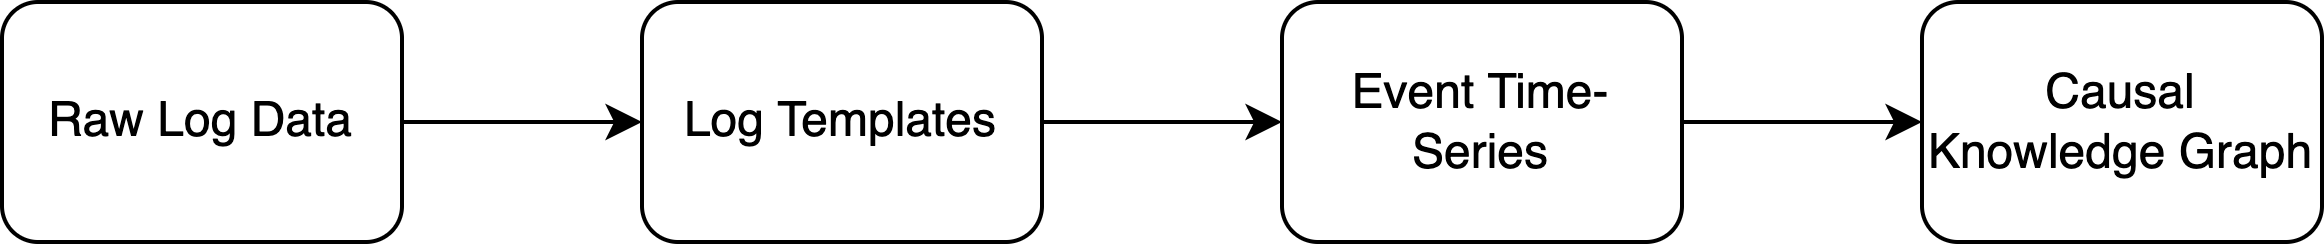
\includegraphics[width=\textwidth]{figures/structure.png}
    \caption{The general processing flow.}
\end{figure}
The overview of causal analysis literature is shown in Figure \hyperref[fig:structure]{1}. This analysis flow follows the main existing approaches \cite{jarry2021quantitative,jia2017approach,kobayashi2017mining,lou2010mining,otomo2019latent}.\newline

The input data is a set of raw log messages, including timestamps, source parameters, and free-format messages. First, we generate log templates of the log messages with some template generation algorithms to aggregate the messages into a set of event time-series in a time bin. We define a node of causal discovery as an event time-series, corresponding to one per device per log type (log template). Some approaches also apply time-series preprocessing to remove periodicity and regularity, which causes false causality detection \cite{jarry2021quantitative,kobayashi2017mining}. Finally, we conduct causal discovery with the event time-series input to get the causal knowledge graph.
\section{Log Templates Generation}
\label{sec:3}
There is one challenge to be carefully considered to apply causality discovery algorithms to log data.
\begin{figure}[h]
\centering
    \label{fig:log-template}
    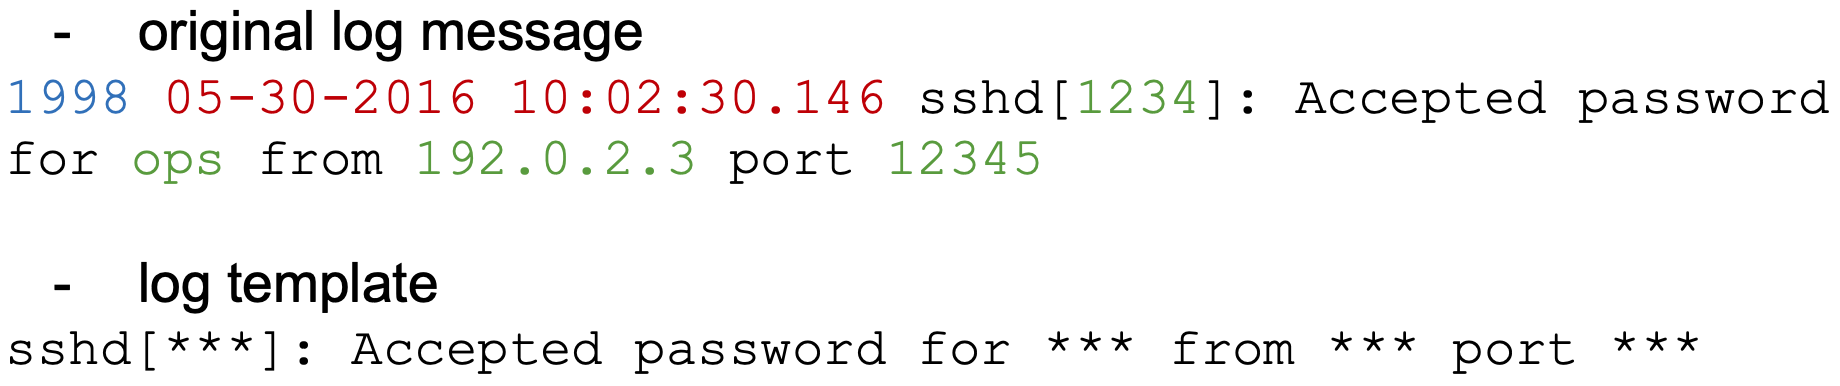
\includegraphics[width=0.85\textwidth]{figures/log_template.png}
    \caption{Example of log template.}
\end{figure}
Raw log messages cannot be analyzed directly with statistical approaches because they are string, not numeric. The content of a log record is an unstructured free-text written by software developers, which makes it challenging to structure. Log messages often contain two types of information: one is a free-form text string used to describe a recorded program event; the other is parameters used to express some essential characteristics of the current task. The log template is a log format, the variables of which are replaced by parameter placeholder *. So we need to extract log templates from the original log messages except for IDs and timestamps. The figure \hyperref[fig:log-template]{2} is an example of a log message and the corresponding log template. In this example, variables such as process ID, user name, IP address, and port number are replaced by stars.\newline

However, Kobayashi et al. \cite{jarry2021quantitative,kobayashi2017mining} consider one more issue that appears by log messages generation. The distribution of log appearances is long-tailed; like daily processes, some events occur much more frequently than others, like error logs. Such a periodic log template represents regular daily events caused by an event timer. This difference in frequency significantly affects the algorithms. Indeed, the algorithms detect more edges from frequent events while hiding important relations of minor events. To avoid this, they propose to remove events that appear frequently but are less critical in troubleshooting. For this purpose, the authors use the following two methods: a Fourier analysis to find periodic events of large intervals and linear regression analysis for short intervals.\newline

Traditional log parsing techniques rely on human experts' regular expressions designed and maintained. Large systems with various software and hardware components render it intricate to support this manual effort. Thus, automated log parsing is essential due to its practical relevance to maintenance systems. Parsing techniques can be distinguished in the following classes based on various aspects, including technological, operation mode, and preprocessing \cite{nedelkoski2020self}: 
\begin{enumerate}
\item \textit{Clustering}. The central assumption in this class of methods is that the message types coincide in similar groups. Various clustering methods with proper string matching distances have been used. LKE applies weighted edit distance with hierarchical clustering to do log key extraction and a group splitting strategy to fine-tune the obtained log groups \cite{fu2009execution}. LogMine creates a hierarchy of log templates that allows the user to choose the description level of interest \cite{hamooni2016logmine}.
\item \textit{Frequent pattern mining} assumes that a message type is a systematic set of tokens that appear throughout the logs. The procedures involve creating frequent sets, grouping the log messages, and extracting message types. Representative methods for this class are LFA \cite{nandi2016anomaly} and LogCluster \cite{xu2009detecting}.
\item \textit{Evolutionary}. This class member is MoLFI, which uses an evolutionary approach to find the Pareto optimal set of message templates \cite{messaoudi2018search}.
\item \textit{Log-structure heuristics}. These methods exploit different properties that emerge from the structure of the log. The state-of-the-art Drain assumes that the words do not vary too much at the beginning of the logs \cite{he2017drain}. It uses this assumption to create a tree of fixed depth that can be easily modified for new groups. As a result, it produces the best results among the different adopted techniques \cite{zhu2019tools}.
\item \textit{Longest-common sub-sequence} uses the longest common sub-sequence algorithm to extract log patterns from incoming log messages dynamically. Here the most representative algorithm is Spell \cite{du2016spell}.
\item \textit{Neural}. The key idea for this parsing is that the correct prediction of the masked word means that the word is a part of the log template; otherwise, it is a log parameter. The most representative approach is a self-supervised method NuLog \cite{nedelkoski2020self}, which utilizes the transformer architecture \cite{devlin2018bert}.
\end{enumerate}
\section{Event Time-Series Creation}
\label{sec:4}
\begin{figure}[H]
\centering
    \label{fig:ts-creation}
    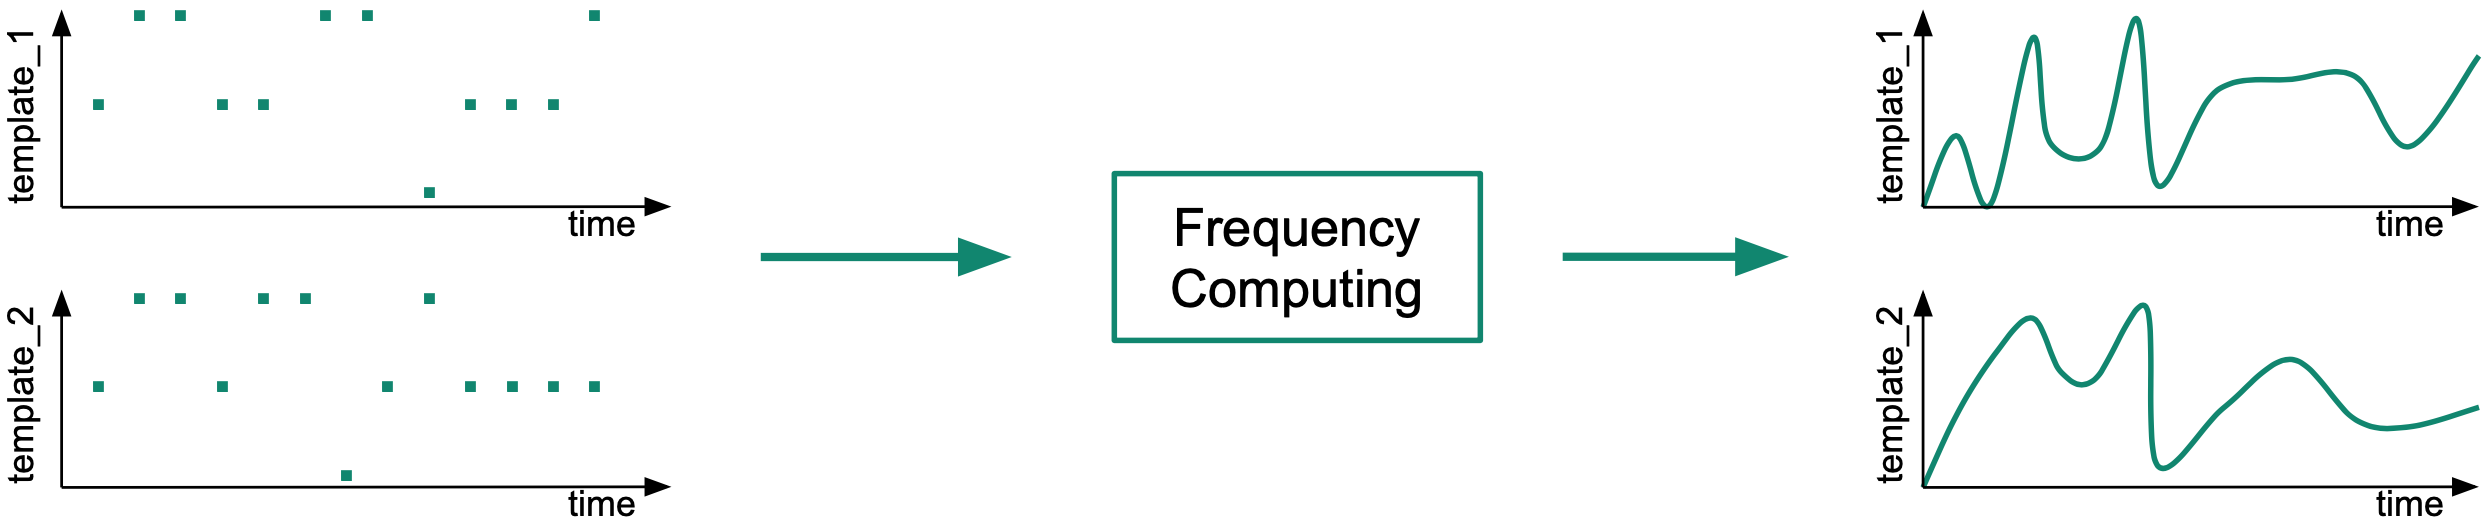
\includegraphics[width=\textwidth]{figures/ts_creation.png}
    \caption{The time-series creation flow.}
\end{figure}
After extracting the log templates, we construct a set of event time-series generated by each log template from all log data. In other words, we compute the frequency of log templates, that is, the number of appearances of one log template in each time bin (see also Figure \hyperref[fig:ts-strategies]{3}). This transformation from log space to metric space helps us run causal inference algorithms directly on information from log data \cite{jia2017approach}.
\begin{figure}[H]
\centering
    \label{fig:ts-strategies}
    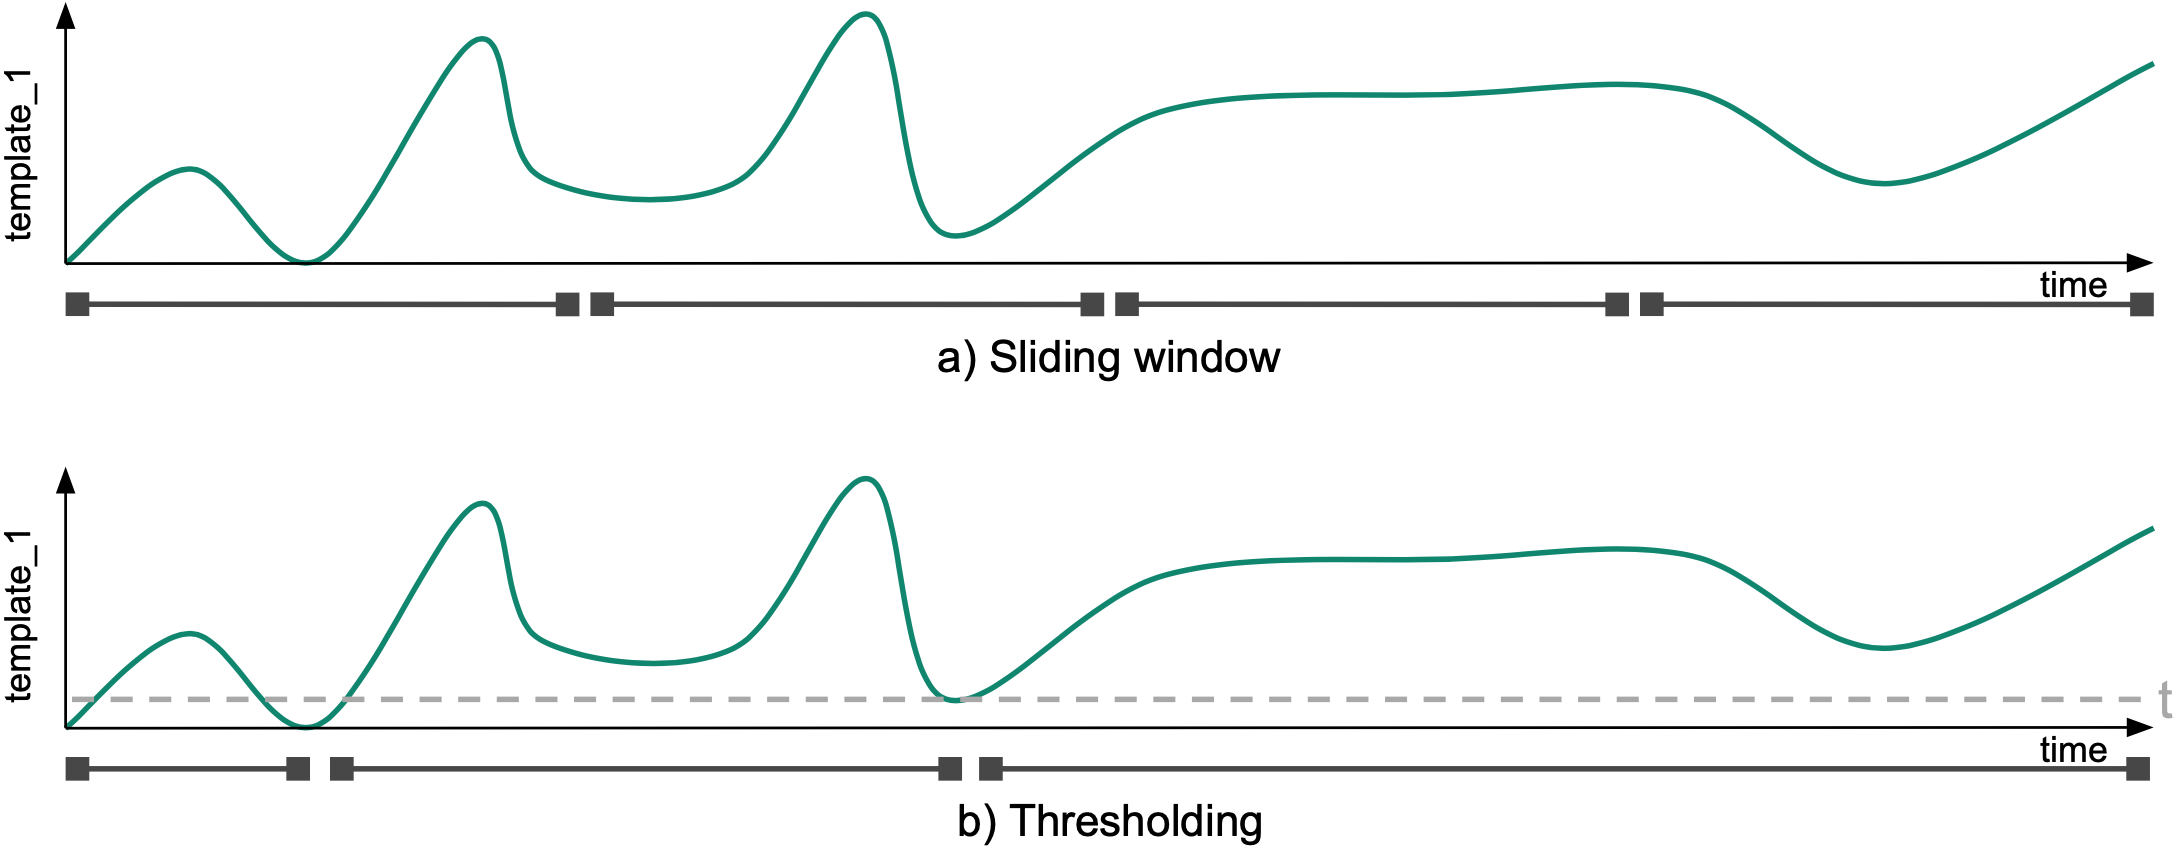
\includegraphics[width=\textwidth]{figures/ts_strategies.png}
    \caption{The time-series modeling strategies.}
\end{figure}
There are two main strategies for treating time-series data \cite{glymour2019review}. One is to partition the data into non-overlapping equals windows and take the measurements in each unit as a data analytic unit (see also Figure \hyperref[fig:ts-strategies]{4 a}). Another is to assume or estimate the number of lagged effects and treat all observations separated by no more than that number of log templates $\tau$ (threshold) as a data analysis unit (see also Figure \hyperref[fig:ts-strategies]{4 b}). Each strategy has its disadvantages. The sliding window method necessarily omits relations across windows, and results may vary with the choice of window size. In the second method, the time units are not all independent, but most units are.
\section{Causal Inference Algorithms}
\label{sec:5}
Causal inference consists of two key ideas to estimate causal relations between events: removing spurious correlations and determining directions of causal edges. This section explains the basic idea of causal inference and existing approaches to analyzing log data. I will illustrate three main classes of algorithms: constraint-based, score-based, and functional-based. In this paper, I selected one prominent algorithm from each group. But if we start exploring the multivariate time-series analysis literature regarding causality, we will likely come across the term Granger causality. This paper will also explain Granger causality and why it is not the true causality, unlike "cause and effect" relationships.
\subsection{Constraint-based}
The primary and main idea of a theory of inferred causation is to present a causal structure among variables in an acyclic directed graph (DAG) called a causal graph in which arrows indicate causal orders, where each node represents a feature from the data set \cite{pearl2009causality}. If we want to say that $X$ causally influences $Y$ and not the other way around, we simply write $X \rightarrow Y$. \newline

But firstly, I will define the statistical decision procedure, a hypothesis test for \textbf{conditional independence}, to reveal causality from correlation. Conditional independence is usually formulated in terms of conditional probability. Assume three events: $X$, $Y$, and $Z$. $X$ and $Y$ are conditionally independent for given $Z$ if
\begin{equation}
P(X \mid Y, Z)=P(X \mid Z)
\end{equation}
where the events $X$ and $Y$ are independent as long as $Z$ appears. In other words, since the probability of $X$ given $Z$ is the same as the probability of $X$ given both $Y$ and $Z$, this equality expresses that $Y$ contributes nothing to the certainty of $X$. With the idea of conditional independence, we can remove pseudo causality/spurious correlation in this way. \newline
\begin{figure}[ht]
\centering
    \label{fig:ci-example}
    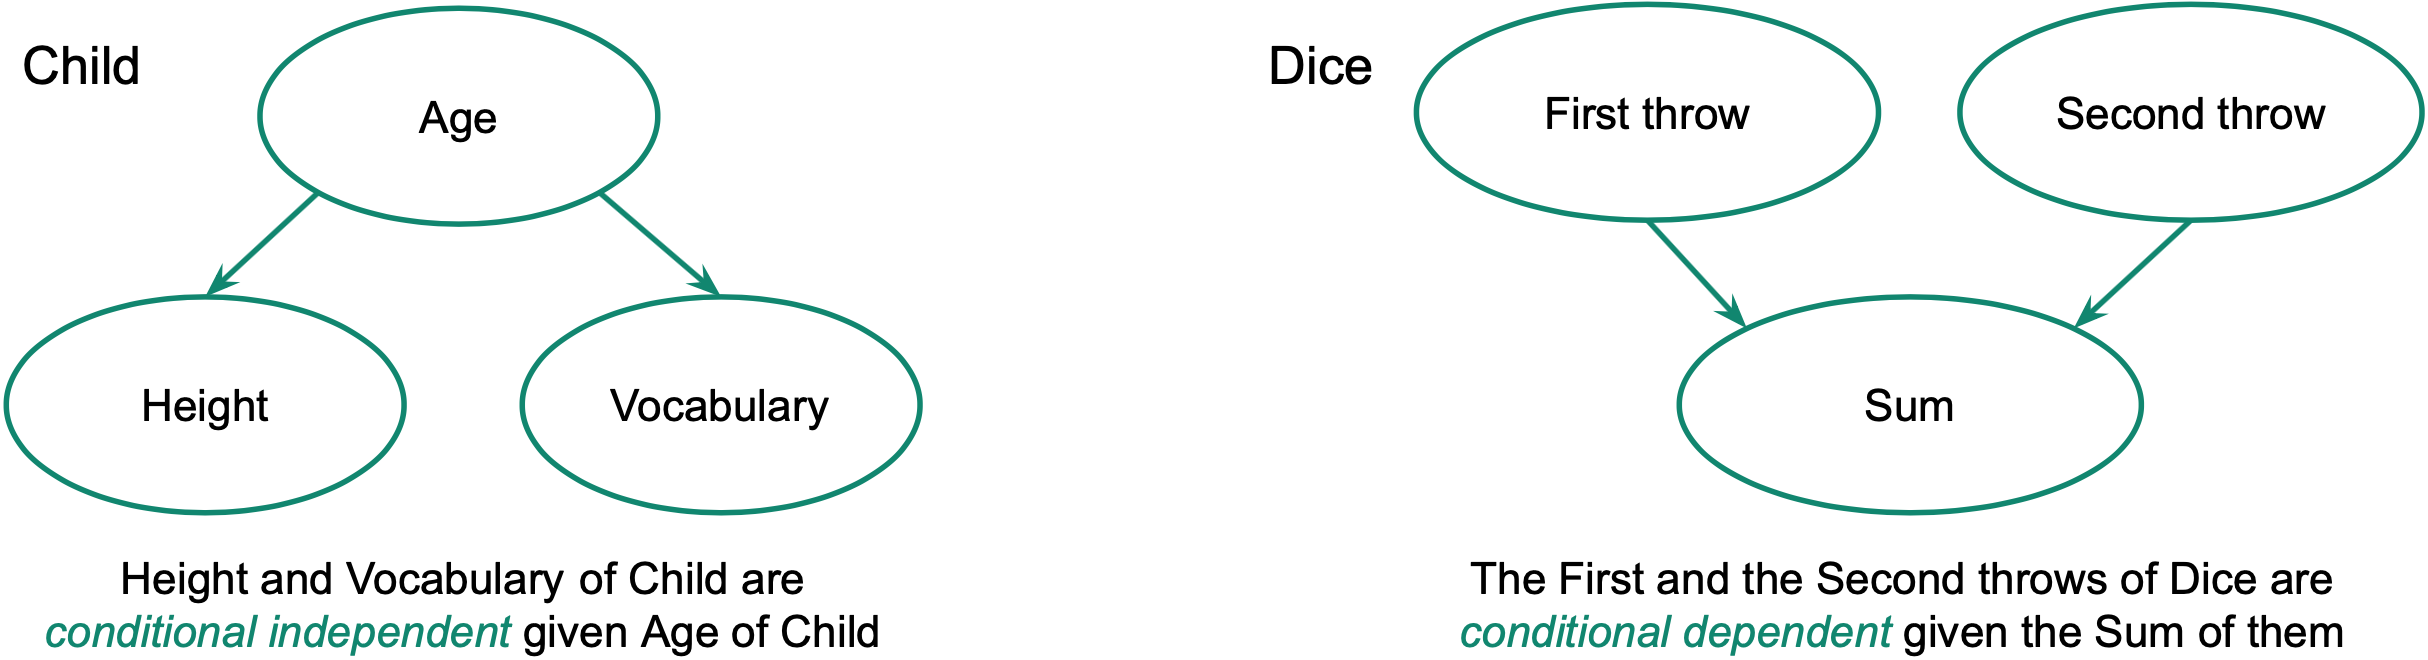
\includegraphics[width=\textwidth]{figures/ci_example.png}
    \caption{The conditional independence examples.}
\end{figure}

To clarify, neither conditional independence of two variables implies their independence, nor the other way around I prepared two counterexamples (see also Figure \hyperref[fig:ci-example]{5}). The first example is about a child. Firstly, we focus only on two events: the child's height and the number of words that the child knows. It seems when the first parameter is high, the second is high too. So they are not independent. But if we provide the child's age. We will see the dependence between age and height and between age and vocabulary. But if we go back to the probability definition, we can say that height and vocabulary of the child are conditionally independent given the child's age. The second example is about dice. We can throw dice twice and get two independent results. But if we provide the parameter like the sum of these throws, we will see the pairwise dependency between each throw and sum. And we can say in this case that the first and the second throw of dice are conditionally dependent given their sum. \newline

One can consider three methods for testing conditional independence in practice \cite{kobayashi2017mining}:
\begin{enumerate}
\item The \textit{G-square test} is a method to evaluate conditional independence of binary or multi-level data based on information theory, using conditional cross-entropy ($CE$) and the data length ($m$). The G-square statistic $G^2$ is defined as:
\begin{equation}
G^{2}=2 m C E(X, Y \mid Z)
\end{equation}
\item The \textit{Fisher-Z test} evaluates the conditional independence of continuous data based on Pearson’s correlation coefficient ($r$) and the data length ($m$). The statistic $Zs$ is defined as:
\begin{equation}
Z s=\frac{\sqrt{m-|Z|-3}}{2} \log \frac{1+r}{1-r}
\end{equation}
\item The \textit{conditional mutual information test} is a form of evaluating conditional independence of discrete and continuous data based on information theory, using conditional entropy and probability function. The conditional MI test $I$ is defined as:
\begin{equation}
I(X , Y \mid Z)=H(X \mid Z)-H(X \mid Y, Z)=E\left[\log \frac{p(X, Y \mid Z)}{p(X \mid Z) p(Y \mid Z)}\right]
\end{equation}
\end{enumerate}
In experiments with log data, Kobayashi et al. \cite{kobayashi2017mining} found that Fisher-Z leaves more false-positive edges and takes more time than the G-square test. \newline

This class of algorithms relies on four assumptions to develop the correct DAG structure. All the independencies in a graph need to be under the conditional independence criterion \cite{nogueira2021causal}:
\begin{enumerate}
\item \textit{Causal Markov} – if two variables are conditional independent of each other, given all their intermediate variables, these variables must be unconnected.
\item \textit{Causal Faithfulness} – if two variables are conditional dependent, connecting those variables must be an edge.
\item \textit{Causal Sufficiency} – all the common causes of a pair of variables are measured (there are no hidden/external causes).
\item \textit{Independency} –  no variable is an (indirect) cause of itself.
\end{enumerate}

Constraint-based methods for causal discovery have the advantage that it is generally applicable. Still, the disadvantages are that faithfulness is a strong assumption and that it may require substantial sample sizes to get good conditional independence tests.
\begin{figure}[H]
\centering
    \label{fig:pc}
    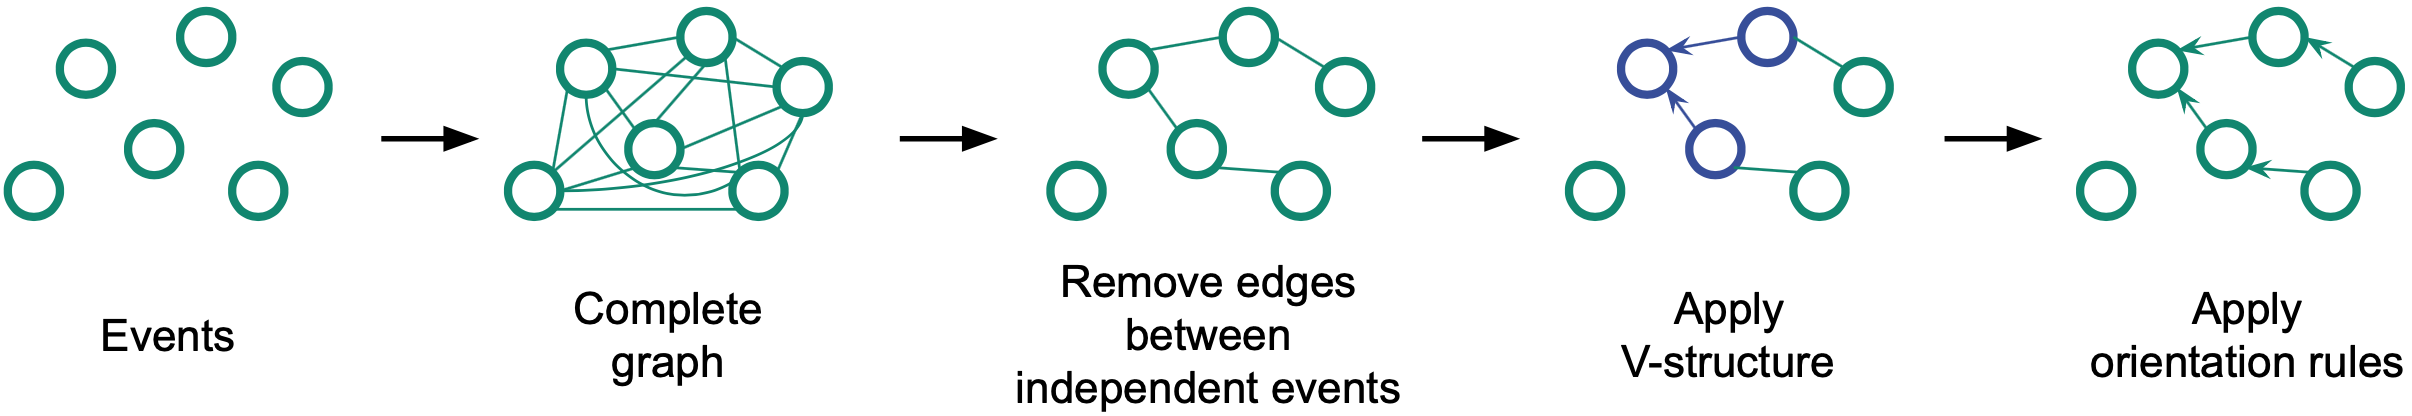
\includegraphics[width=\textwidth]{figures/pc.png}
    \caption{The PC algorithm flow.}
\end{figure}
\textbf{PC Algorithm} \cite{spirtes2000causation}. One of the most common algorithms in literature is the PC algorithm, which aims to find the graphs representing precisely the independent relationships present in the data through hypothesis tests. The PC algorithm consists of four steps (see also Figure \hyperref[fig:pc]{6}). We start with a set of created from logs event time-series. Then we construct a complete (fully connected undirected) graph from events. Next, we eliminate edges between conditionally independent nodes by analyzing all pairs. Then, the triple of nodes (in blue color on Figure \hyperref[fig:pc]{6}) is called V-structure with the following orientations of edges. So we look for the V-structures of nodes and determine edge direction. Finally, we determine other edge directions with the orientation rules defined by the algorithm. But some edges can be undirected even after applying the PC algorithm if one does not have enough information to determine edge directions. In other words, in the first two steps, we estimate a skeleton graph that is an undirected causality graph with the idea of causal inference. In the last two steps, we determine the directions of the detected edges with established rules. The V-structure is the main rule to decide on the direction of an edge. For example, there are three events $X$, $Y$, $Z$ that are a part of a graph $X-Y-Z$. $X$ and $Y$ are correlated, and $Y$ and $Z$ are connected. One obtains a causal relationship $X \rightarrow Y \leftarrow Z$ if $X$ and $Z$ are not conditionally independent for $Y$. The remaining undirected edges can be oriented by using experimental data or knowledge about data sources. \newline

In practice, the PC algorithm has some variations. One of these algorithms is the PC-stable \cite{colombo2014order}. This algorithm solves the problem that the traditional PC is dependent on the order in which the events are given to the algorithm. This adaptation modifies how the algorithm creates the skeleton: in each level, the event that should be removed are also saved in a queue and are only permanently removed in the next iteration. PC-simple modification is based on local causality discovery \cite{buhlmann2010variable}. The difference is that it only analyses the strongly related variables to the selected target variable (that is, it does not analyze or create the network with the remaining variables). This algorithm was developed to deal with high-dimensional data. The HITON-PC is a mixture of two of the previously presented algorithms, PC-stable and PC-simple \cite{aliferis2003hiton}. Another extension is the parallel-PC which is a parallel adaptation of PC \cite{le2016fast}. This parallelization is done in the conditional independence tests performed at each level of the algorithm. These tests are grouped and distributed in different cores. The MPC modifies the original orientation rules by adding a new rule that prevents the creation of cycles (although DAGs do not allow cycles, PC does not explicitly prevent their creation) \cite{tsagris2019bayesian}.
\subsection{Score-based}
These algorithms differ from the previous ones because they are based on the greedy strategy to make the locally optimal choice at each stage and compare the interim graphs through the Bayesian Information Criterion (BIC) \cite{stoica2004model}. These algorithms are usually costly in terms of performance since they have to score every model.
\begin{figure}[H]
\centering
    \label{fig:ges}
    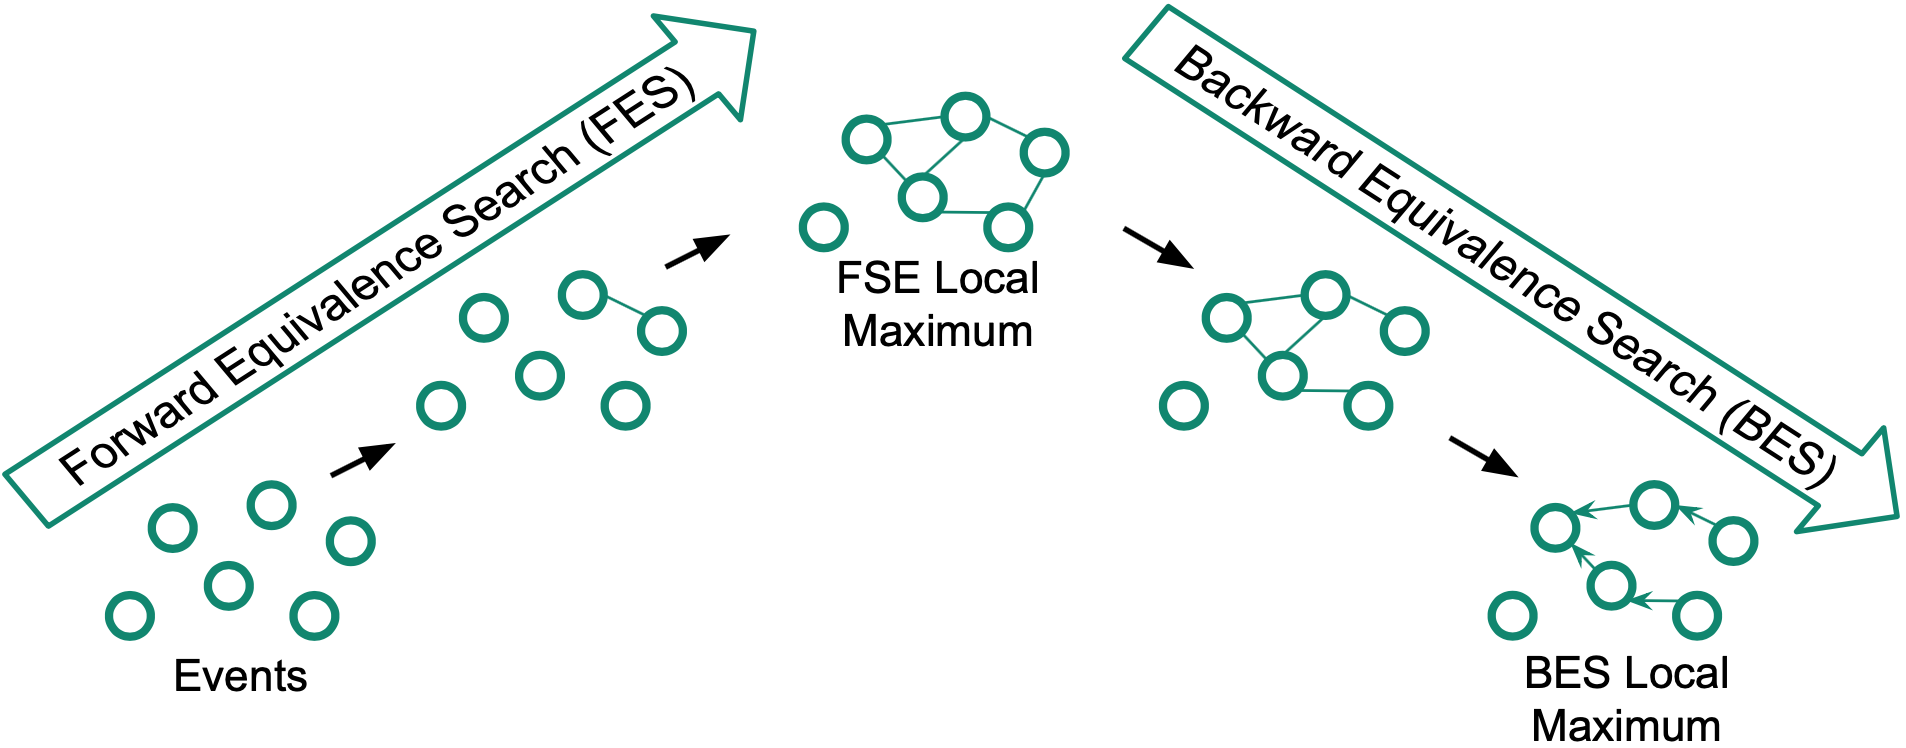
\includegraphics[width=\textwidth]{figures/ges.png}
    \caption{The Greedy Equivalence Search flow.}
\end{figure}
\textbf{Greedy Equivalence Search (GES)} \cite{chickering2002optimal}. The GES algorithm generally consists of two phases (see also Figure \hyperref[fig:ges]{7}). In the Forward Equivalence Search (FES) phase, the algorithm starts with a set of events. Then at each step, as a decision is made as to whether adding an edge to the graph will increase the score BIC, the edge that most improves the score is added until the algorithm reaches a local maximum. This algorithm analyses all possible node-neighbors each time. Then the second phase of the algorithm begins, which asks, edge by edge, which edge removal if any, will most improve the score until it reaches a local maximum. But in this phase, the direction of edges is also taken into account. \newline
	
In practice, the GES algorithm also has some variations. One example is the Greedy Interventional Equivalence Search (GIES), in which, besides the FES and BES phases, there is a third phase called the Turning Step \cite{hauser2012characterization}. In this extra phase, the algorithm iterates all possible orientations of edges without losing edges or creating new ones so that the previous graph can be reconstructed by only changing arrows. This phase was added with the intent to enhance estimation. Another example is the Fast Greedy Equivalence Search (FGS) \cite{ramsey2017million}. This algorithm uses parallelization to optimize the original GES and applies a limited faithfulness assumption.
\subsection{Functional-based}
\begin{figure}[H]
\centering
    \label{fig:x-y}
    
\includegraphics[width=0.3\textwidth]{figures/x_y.png}
    \caption{The simple causal graph.}
\end{figure}
For the introduction to this class, I will start with the definition of the problem by determining the causal direction in the two-variable case, where no conditional independence relationship is available. A fundamental issue is given two variables $X$, $Y$ (see also Figure \hyperref[fig:x-y]{8}), how to distinguish cause from effect. We need to find a way to capture the asymmetry between them to do so. Functional-based approaches represent the effect $Y$ as a function of the direct causes $X$ and some unmeasurable factors or noise:
\begin{equation}
Y = f(X) + E
\end{equation}
where $E$ is assumed to be independent of $X$, the function $f$ explains how $Y$ is generated from $X$. We assume that the transformation from $(X, E)$ to $(X, Y)$ is invertible, such that $E$ can be uniquely recovered from the observed variables $X$ and $Y$. So, these algorithms consider the data asymmetry effect induced by the causal directions \cite{glymour2019review}.
\begin{figure}[H]
\centering
    \label{fig:fb-example}
    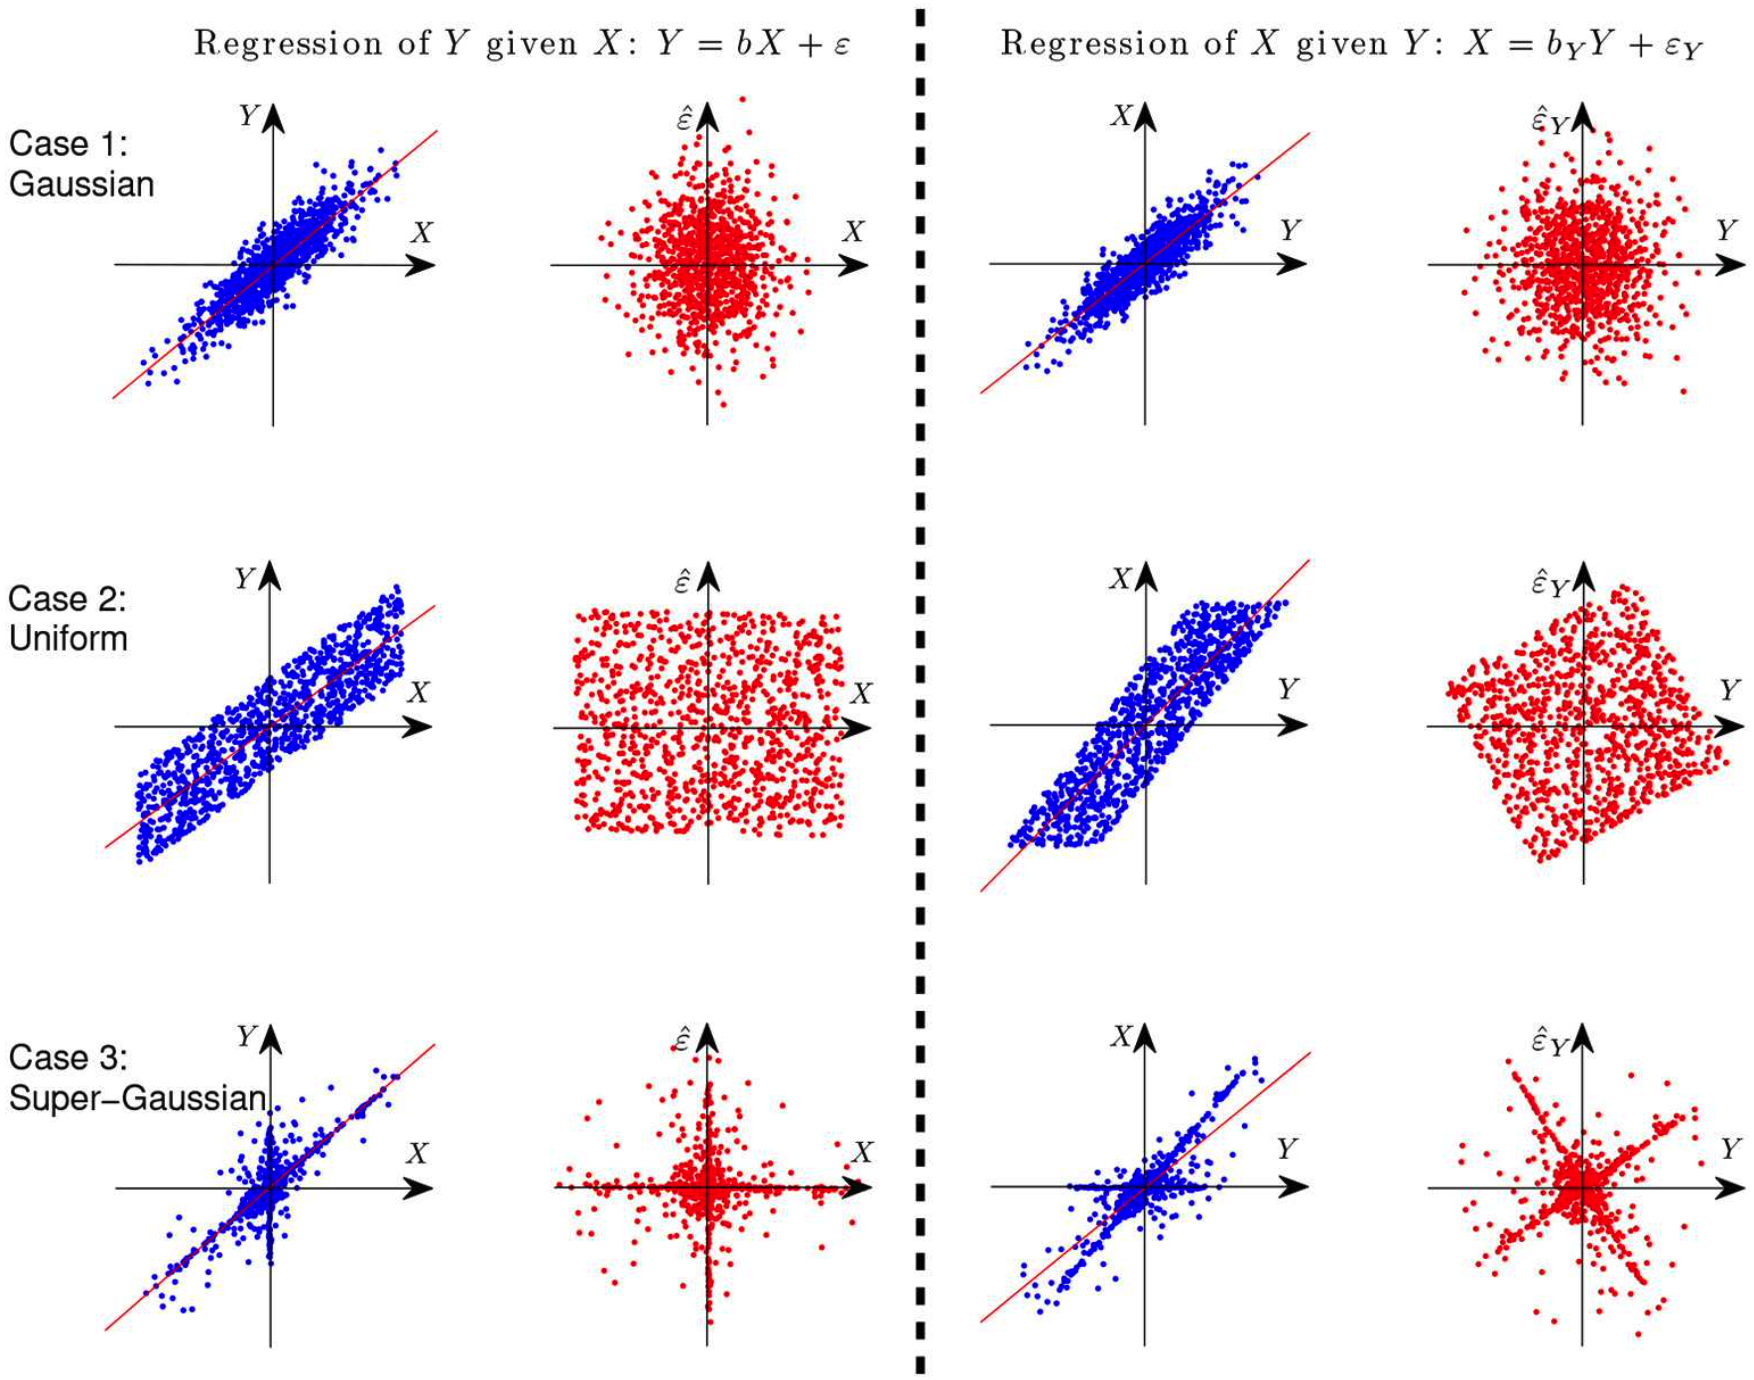
\includegraphics[width=\textwidth]{figures/fb_example.png}
    \caption{The illustration of causal asymmetry between two variables with linear relations.}
\end{figure}
What does it mean data asymmetry effect? Under the above assumptions, we fit the functional-based test and then check for independence between the estimated noise term and the hypothetical cause. So the direction which gives an independent noise term is considered plausible. The figure \hyperref[fig:fb-example]{9} is a simple example of why it is possible to identify the causal direction between two variables in the linear case, $f$ is the linear function. Assume $Y$ is generated from $X$ in a linear form, where $E$ is independent of $X$. Columns 1 and 3 are the scatter plots of the two variables $X$ and $Y$, the red line is the linear regression of $Y$ on $X$, columns 2 and 4 are the predictor and regression residual for two different regression tasks. The three rows correspond to different settings: $X$ and $E$ are both Gaussian (case 1), uniformly distributed (case 2), and distributed according to some super-Gaussian distribution (case 3). In the last two cases, $X$ and $E$ are non-Gaussian, and one can see clearly that for regression of $X$ given $Y$ (the backward direction), the regression residual is not independent of the predictor anymore, although they are uncorrelated by the construction of regression. In other words, in those two situations, the regression residual is independent of the predictor only for the correct causal direction, giving rise to the causal asymmetry between $X$ and $Y$. As a result, based on this asymmetry, we can conclude that $X$ is the cause of $Y$ \cite{glymour2019review,goudet2018learning}.\newline

In practice, there are two directions of functional-based methods. The first way uses a linear function (e.g. Linear Non-Gaussian Acyclic Model (LiNGAM) \cite{shimizu2006linear}), and the second way — non-linear functions (e.g. Post-nonlinear (PNL) Causal Model \cite{zhang2012identifiability}). In the linear, non-Gaussian, and acyclic model (LiNGAM), a function is linear, and at most one of the noise term $E$ and cause $X$ is Gaussian. In PNL, the effect $Y$ is further generated by a post-nonlinear transformation on the non-linear effect of the cause $X$ plus noise term $E$, where both functions are non-linear and outer function is assumed to be invertible.
\begin{figure}[H]
\centering
    \label{fig:fb-flow}
    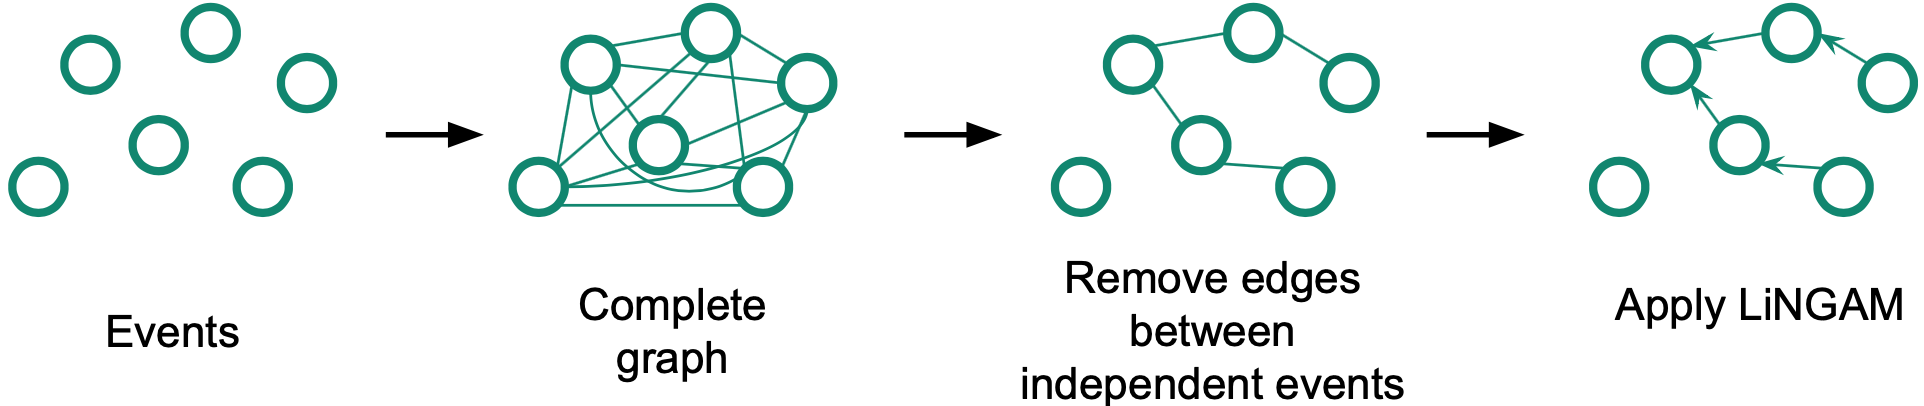
\includegraphics[width=\textwidth]{figures/fb_flow.png}
    \caption{The functional-based approach flow.}
\end{figure}
To apply this group of algorithms to our case, we first need to create the graph skeleton with a PC algorithm (see also Figure \hyperref[fig:fb-flow]{10}). And then, we estimate the orientation of edges based on the data asymmetry effect. Kobayashi et al. \cite{jarry2021quantitative} found that MixedLiNGAM discovers ten times more causal edges than the PC algorithm. 
\subsection{The Granger Causality}
\begin{figure}[ht]
\centering
    \label{fig:granger}
    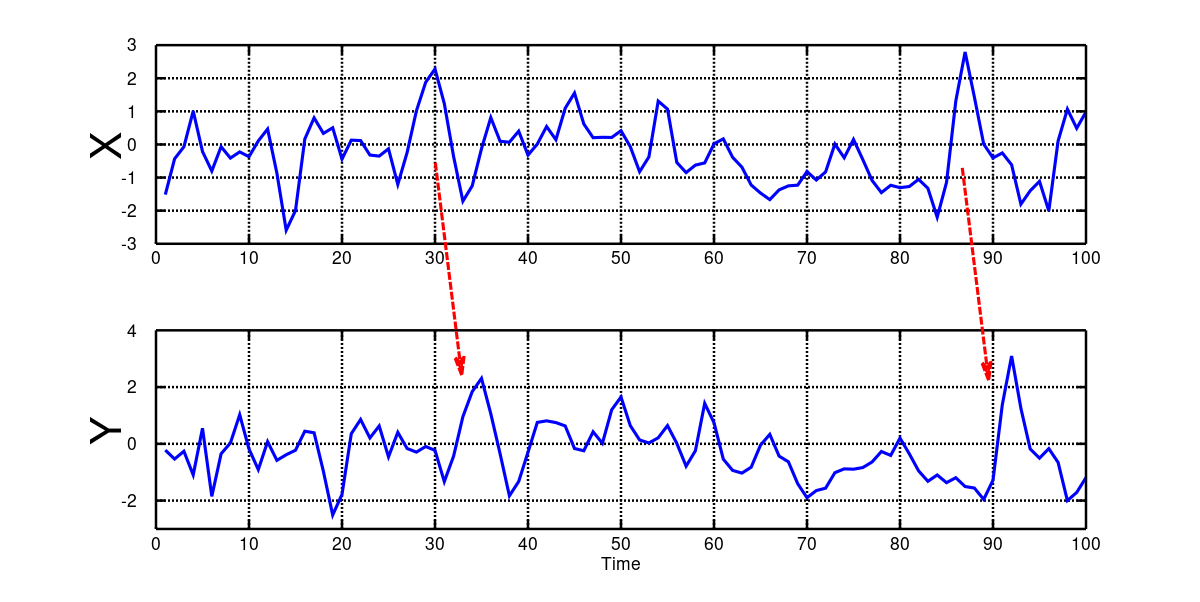
\includegraphics[width=\textwidth]{figures/granger.png}
    \caption{The time-series $X$ Granger-causes time-series $Y$.}
\end{figure}

The Granger causality test is a statistical hypothesis test for determining whether one time-series is helpful in forecasting another. The figure \hyperref[fig:fb-example]{11} is an example where the patterns in $X$ are approximately repeated in $Y$ after some time lag (two arrows). Thus, past values of $X$ can be used to predict future values of $Y$. Clive Granger defined the causality relationship based on two principles: the cause occurs before the effect, and the cause has unique information about the future values of its effect \cite{granger1980testing}.\newline

To test the Granger causality, we need to augment the autoregression model of one time-series $Y$ by including lagged values of another time-series $X$: 
\begin{equation}
y_{t}=c+\epsilon_{t}+\sum_{i=1}^{p} \alpha_{i} y_{t-i}+\sum_{i=1}^{p} \beta_{i} x_{t-i}
\end{equation}
So we need to determine if any lags of $X$ are statistically significant in our model of $Y$. We can do this using a Wald test F-statistic for linear restrictions. The Wald test is based on the relatively simple premise that we wish to compare the performance of a restricted model for $Y$, which excludes $X$, against an unrestricted model for $Y$, which includes $X$. The null hypothesis that $X$ does not Granger-cause $Y$ is accepted if and only if no lagged values of $X$ are retained in the regression according to an F-statistic.\newline

However, Granger stressed that some studies using "Granger causality" testing in areas outside economics reached "ridiculous" conclusions. \textit{"Of course, many ridiculous papers appeared,"} he said in his Nobel lecture \cite{granger2004nobel}. Thus, the Granger causality is not the true causality. It does not provide any insight into the relationship between the variable and is helpful only in the forecasting case. Moreover, time is the key parameter in this approach. However, the timestamp of system logs or just time-series is not always reliable for determining causal directions due to time synchronization errors between devices, jitter, and network failures \cite{kobayashi2017mining}. This kind of approach has other limitations. One of them is that the Granger causality gives only information about linear features. Besides this, one more is that the variables must be stationary. Finally, this approach is very dependent on the observations that we are dealing with \cite{seth2007granger}.

\section{Conclusion}
\label{sec:6}
Understanding causal relations helps construct interventions to achieve particular objectives and makes predictions under interventions. The growing accumulation of vast amounts of data necessitates the development of scalable automatic causal search algorithms. This paper has reviewed the step-by-step solution to the time-series data causal discovery challenge. Specifically, I first discussed the preparation phase for the set of log messages because causal discovery algorithms require a suitable structure as input. In this part, I discussed the log parsers and two strategies to create time-series data from log messages. Then, I described four classes of causal inference algorithms: constraint-based, score-based, functional-based methods, and the Granger causality test. If you have a task to explore causality, you can choose one of the proposed algorithms for each step. As a result, you get your algorithm pipeline. Future research directions include solving the issue of missing relationships between two windows by time-series creation and integrating weights to directed edges to discuss the likelihood of causal impact \cite{jarry2021quantitative}.
%
% ---- Bibliography ----
%
% BibTeX users should specify bibliography style 'splncs04'.
% References will then be sorted and formatted in the correct style.
%
\bibliographystyle{splncs04}
\bibliography{mybib}

\end{document}
